\section{Meeting Notes}
\subsection*{Week 2: Meeting on 3/10/2022 at 3pm}
\begin{itemize}
    \item Every member showed up for an hour-long meeting in the library group study room. 
    \item Discussed the project specification and overview of the project and as a group we brainstormed ideas. 
    \item Decided to use Notion as a file sharing tool. Ioanna took the meeting notes. 
    \item Our ideas were a facial recognition app for driverless vehicles, skin disease detector, a carbon footprint calculator, and a computer vision fridge. 
    \item Our aim before the next meeting was to research the feasibility of each idea and pick an idea. 
\end{itemize}

\subsection*{Week 3: Meeting on 10/10/2022 at 1pm }
\begin{itemize}
    \item   Every member showed up for an hour-long meeting in the library group study room. 
    \item   Group unanimously agreed on the smart fridge idea. Alexandre took the meeting notes. 
    \item   We drafted a Moscow graph to agree what features were essential for the operation of the product. 
    \item   Isaac and Yohan agreed to work on the microprocessor and module side of the hardware team and Alfie, Ioanna and Jaime agreed to work on the raspberry pi together. This includes the OpenCV code and the design of the box. Alexandre and Hamzah will both work on the server and website side of the project using AWS. 
    \item   Each group was assigned to research what was needed in each of their sections.  
\end{itemize}

\subsection*{Week 3: Meeting on 12/10/2022 at 2pm }
\begin{itemize}
    \item Everyone Turned Up (6 in person and 1 online (due to Covid)) in the maker space. Isaac took the meeting notes. 
    \item As a group we compared what research we had done up until that point and agreed on what components we were using. 
    \item We also built a block diagram, so we knew what dependencies each team had on another. 
    \item The design brief was discussed, and the sections were split between the members. Isaac was assigned to the overview, Yohan and Ioanna were assigned to the technical overview, Hamzah was assigned to the sustainability section, Jamie and Alfie did the Project management and Alexandre was responsible for the appendices.  
\end{itemize}
    
\subsection*{Week 4: Meeting on 17/10/2022 at 2pm }
\begin{itemize}
    \item This was an online meeting to talk briefly about the progress of the design brief. 
    \item Parts of the appendices and technical outline were discussed as a group so that we were all on the same page when completing our own sections. 
\end{itemize}

\subsection*{Week 4: Meeting on 19/10/2022 at 2pm }
\begin{itemize}
    \item This meeting was held in the makerspace and the notes were taken by Isaac. 
    \item Alexandre and Hamzah should demonstrations of the first version of their server and website on AWS. 
    \item Jaime presented an early design for the box and Ioanna and Alfie discussed the OpenCV and the raspberry pi's compatibility with the esp32 microprocessor. It was decided that we would use serial communication and send the image data as a base64 string.  
    \item Isaac and Yohan started to place in orders for the components needed for the project.  
    \item We agreed to add our sections of the report to a shared file by Friday 21st of October. 
    \item Alfie, Ioanna and Jaime started coding for the OpenCV, and Isaac and Yohan started to test some of the components which were already available in the makerspace on breadboard. 
    \item Alexandre and Hamzah continued refining the web design and server. 
    \item By the end of the week the weight sensor and HAL sensor were working on breadboard with the correct code outputting the expected results. 
\end{itemize}

\section{Additional Images}
\subsection{Circuit Schematic}
\label{sec:schem}
\begin{figure}[H]        
    \centering
    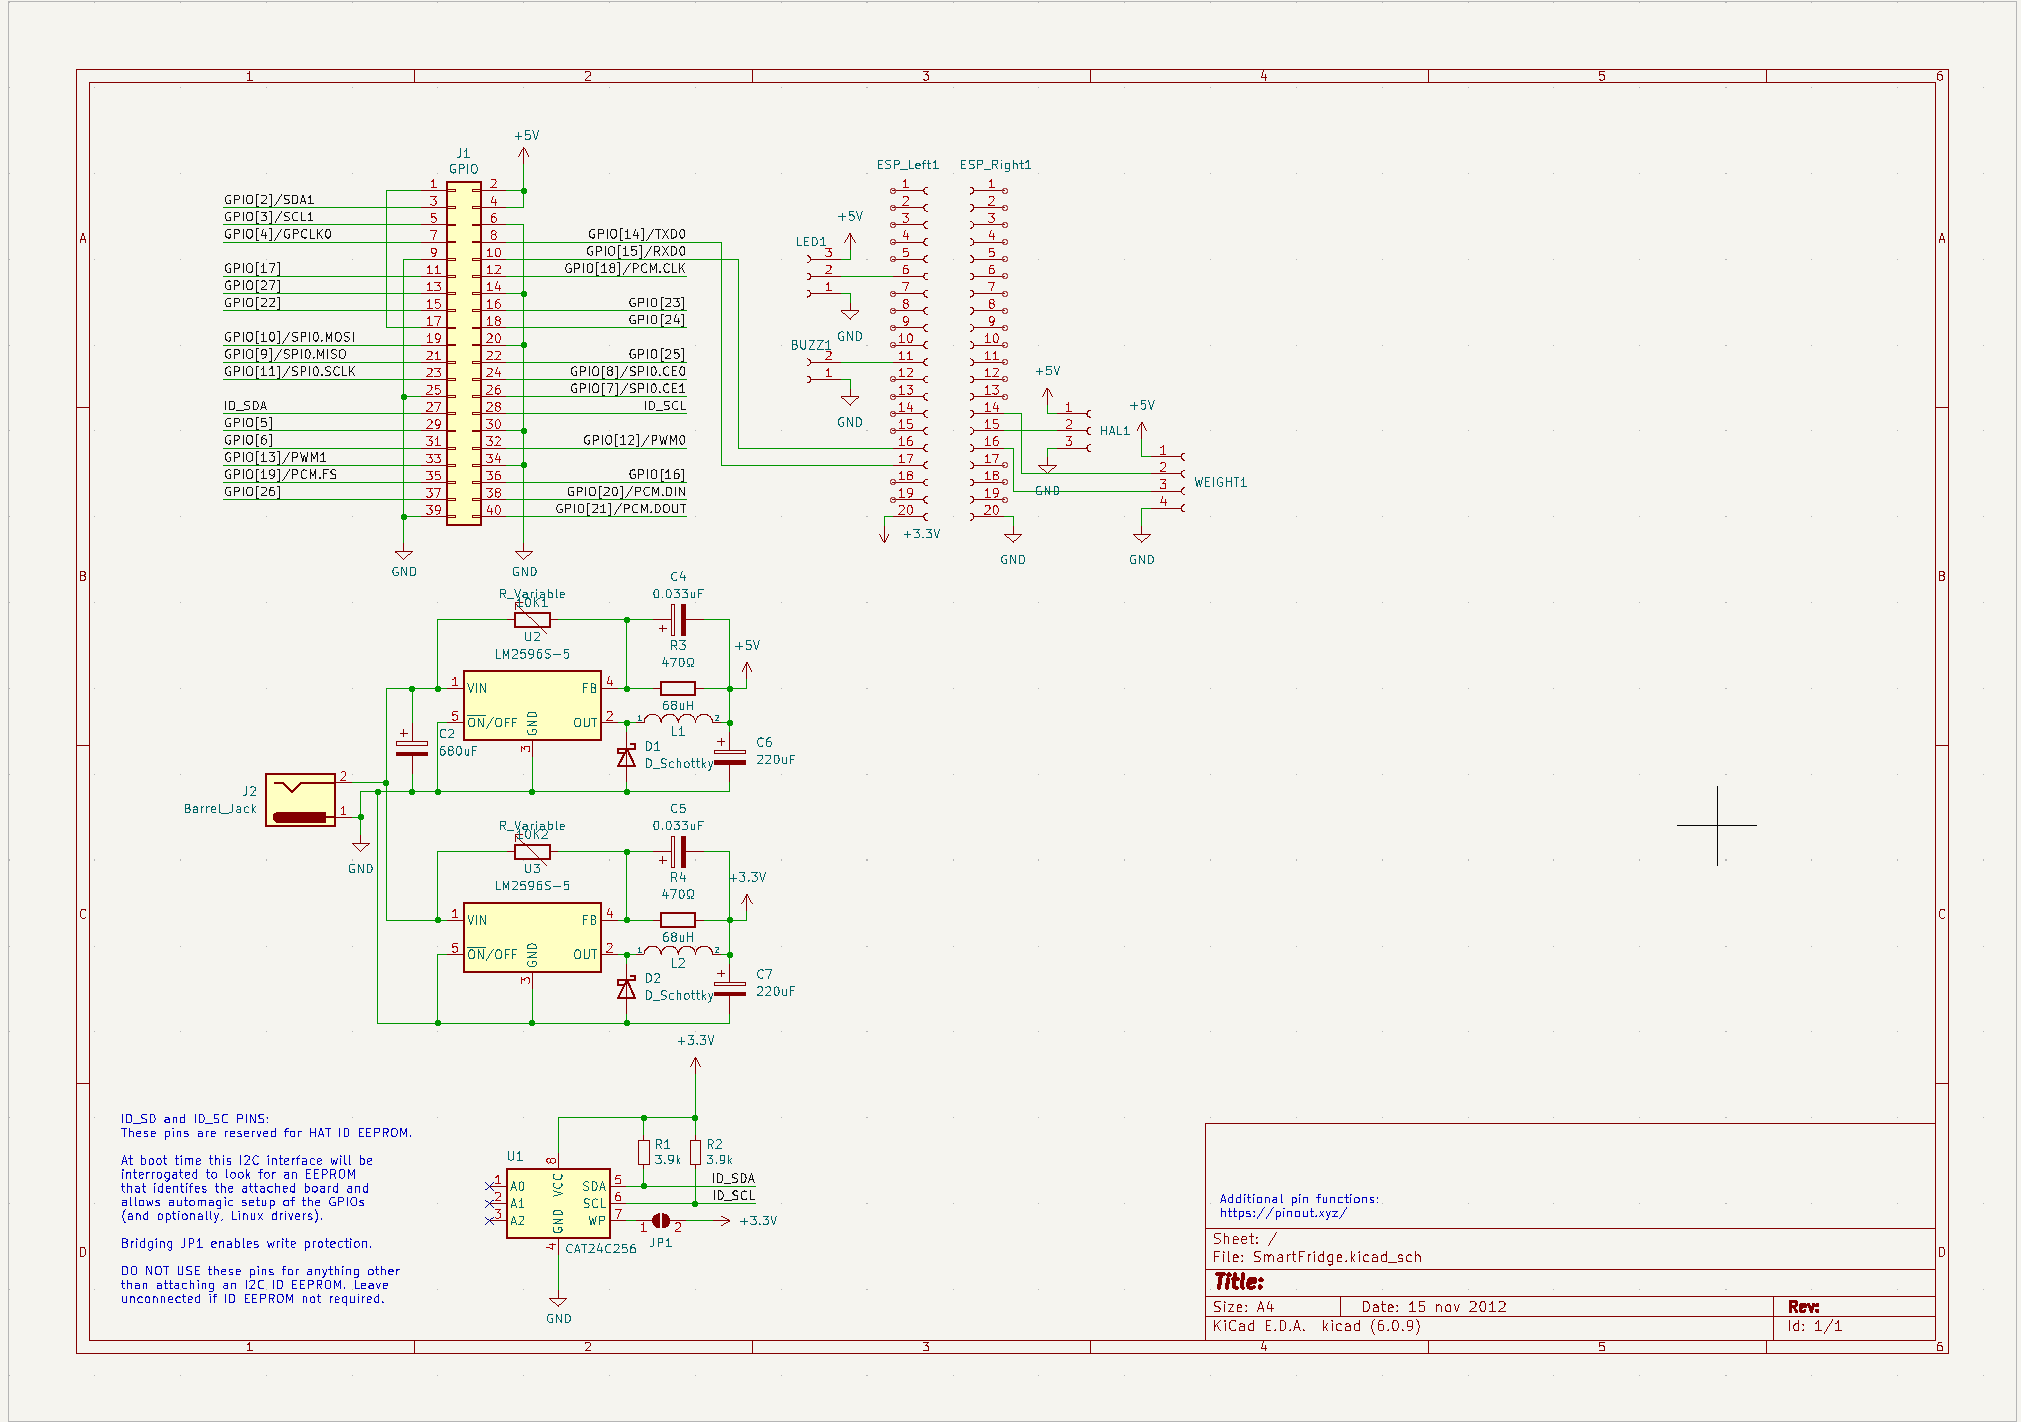
\includegraphics[width=1\textwidth]{Chapter 3/alexandre/schem.png}
    \caption{Schematic for PCB}
\end{figure} 

\section{Additional Forms}






